% vim: ts=4 sts=4 sw=4 et tw=80
\chapter{快速导航}
\label{chap:better_navigation}
\marginpar{53}
同时应付多个文件可能是一件非常麻烦的事, 有时候, 用户可能会花更多的时间来
定位文件, 而不是编辑.

Vim 的处世哲学是不浪费用户的宝贵时间, 所以它提供了许多用于定位文件的方法.

在这一章, 我们将会学习到 Vim 如何帮助我们在多个文件中导航, 无论此时是在
处理 1 个文件, 还是 50 个文件. 其中的某些方法使用标记, 以便于稍后返回到该
区域, 还有些方法使用搜索来定位目标.

这一章包含的内容有:
\begin{itemize}
    \item 在单个文件中更快地导航
    \item 在 Vim 帮助系统中更快地导航
    \item 在多个缓冲区中更快地导航
    \item 使用 Vim 文件浏览器, 以便更快地搜索文件
    \item 文件内搜索
    \item 使用 \texttt{vimgrep} 在多个文件或多个缓冲区中搜索
    \item 使用标记作为导航的工具
    \item 使用符号来得到更好的概览
\end{itemize}

学习后这一章之后, 用户的导航速度将会有质的提升, 在搜索文件时也不会再遇到
什么问题.
\marginpar{54}
\section{在文件内更快地导航}
\label{sec:faster_navigation_in_a_file}

有时候, 即使是一件最简单的工作 --- 比如在一个单独的文件中导航 --- 也有优化
的空间. Vim 提供了几种在文件内导航的方法, 这些方法可以根据文件的内容和组织
结构而加以调整. 其中有些方法非常简单, 而另外一些则比较复杂.

\subsection{基于上下文的导航}
\label{subsec:context_aware_navigation}

在大部分情况下, 正在编辑的文件是有结构的. 如果是普通的文本文件, 那么文件的结
构可以是段落, 语句, 单词, 在另外的一些场合中, 还有可能是函数, 代码块和代码
行.

Vim 支持根据文件的结构, 在文件中跳转. 它还提供了一些按键绑定, 从而可以更
方便地跳转到某个特定的位置上.

让我们来看一些例子:
\begin{itemize}
    \item 在普通的文本文件中移动
    \item 在代码文件中移动
\end{itemize}

\subsubsection{在普通的文本文件中移动}
\label{subsubsec:moving_around_within_a_text_file}

假设用户正在编辑一个普通文件文件, 此时光标正停留在一个句子的中部, 而用户
突然意识到自己忘了把本段的第一个字母大写. 虽然用户可以通过方向键, 或
\texttt{h}, \texttt{j}, \texttt{k}, \texttt{l}, 把光标移到段落的首字母. 然而, 在普通
模式下, 直接按下面这个按键可以得到更好的效果:
\begin{vimcode}
{
\end{vimcode}

按完这个按键之后, 光标已经停在了段落的开头, 或者是段落正上方的空行 (如果
有的话). 现在, 用户可以通过按下 \key{Esc} 进入到普通模式, 再按 \texttt{\{},
把光标移到段落的开始. 与此类似, 用户只要按下和 \texttt{\{} 相对的按键, 即:
\begin{vimcode}
}
\end{vimcode}
就可以把光标移到段落的末尾.

也许用户并不是在段落的末尾工作, 而是在修改段落中的某些错误. Vim 可以记住
用户之前修改过的地方 (实际上, Vim 可以记住最近 999 个被修改过的地方), 因此
用户可以通过询问这些信息, 从而回到正确的地点. 在普通模式下执行下面这个命令:
\begin{vimcode}
g,
\end{vimcode}
\marginpar{55}
执行该命令几次, 就可以遍历之前修改过的地方. 和 \texttt{\{} 一样, 它也有一个相反
的命令, 用于反向遍历之前修改过的地方, 这个命令是
\begin{vimcode}
g;
\end{vimcode}
如果没有更多的地方可供遍历, Vim 就会发出一个警告.

还有一种情况是, 用户并不是在段落的开头忘记了大写字母, 而是在句子的开头, 对此,
Vim 也提供了一对命令, 用来把光标移到句子的开始与末尾, 这对命令是:
\begin{itemize}
    \item \texttt{(}: 移到句子的开头
    \item \texttt{)}: 移到句子的末尾
\end{itemize}

Vim 不希望用户在移动光标上花费太多的时间, 虽然用户可以通过方向键来遍历字母, 从
而在单词间移动, 但是 Vim 还是认为这太浪费按键了. Vim 提供了一组命令, 用于在单词
间移动, 比如:
\begin{itemize}
    \item \texttt{w}: 移到下一个单词的首字母
    \item \texttt{b}: 移到前一个单词的首字母
    \item \texttt{e}: 移到单词的末尾
\end{itemize}
这些命令可以互相组合, 比如, 用户想要移到下一个单词的末尾, 只需要执行:
\begin{vimcode}
we
\end{vimcode}

对于单词的定义, Vim 有两套标准:
\begin{itemize}
    \item 一个 word 由字母, 数字, 破折号, 下划线组成
    \item 一个 WORD 由非空白字符 (除了制表符与空格) 组成
\end{itemize}
前面提到的命令用于 word, 当然, WORD 也会有相应的命令, 只不过使用的是大写形式
(比如用 \texttt{W} 移到下一个 WORD 的首字母).
\marginpar{56}
\begin{warning}
    如果读者希望在一行内多次执行本小节中提到的命令, 只需要在执行命令前加上一个
    数字即可, 这个数字表示命令执行的次数. 例如, \texttt{5w} 表示光标向前移动 5
    个单词.
\end{warning}

\subsubsection{在代码文件中移动}
\label{subsubsec:moving_in_a_code_file}

和普通文本文件相比, 代码文件并没有段落或句子上的概念, 它包含的是大量的结构和块,
其中每一个结构或块都有特定的上下文含义. 一个简单的例子是:
\begin{verbatim}
    if (a == b)
    {
        print "a and b are the same"
    }
\end{verbatim}
代码中, 带有 \texttt{print} 的行在 \texttt{if} 块的上下文环境中.

因为 Vim 深受众多程序员的喜爱, 所以它提供了许多在代码中跳转的命令, 它们的共同
点是, 目标位置和原有位置的代码之间存在着一些语境上的联系.

一个简单的例子可以是 C 语言中的 \texttt{\#if}-\texttt{\#else}-\texttt{\#endif}
代码块, 这三个元素分别处于代码块的开始, 中间, 和结束.

如果用户此时正位于 \texttt{\#if} 所在的行, 执行命令:
\begin{vimcode}
%
\end{vimcode}
就可以跳转到 \texttt{\#else} 所在的行, 此时再按一次 \verb'%', 又会跳转到
\texttt{\#endif} 所在的行, 再按一次 \verb'%' 就会回到最初的 \texttt{\#if}.

Vim 无法识别所有的编程语言的构造, 不过在默认情况下, 它可以识别 C 语言的大部分
结构. 除此之外, 它还可以识别出大部分编程语言的普通代码块 --- 代码块通过圆括号
与花括号定界 (例如, \verb'{' 标出了块的开始, 而 \verb'}' 则表示块的结束).
\marginpar{57}
\begin{warning}
    如果用户希望 Vim 能够识别其他更多语言的构造, 可以通过安装插件
    \texttt{matchit} 来实现, Vim 7.0
    以上的版本已经安装了该插件, 不过也可以到 \url{http://www.vim.org/scripts/}
    上获取.
\end{warning}

通过对程序员如何使用圆括号/花括号的简单了解, Vim 向我们提供了几个有用的导航命令.
也就是说, 只要代码使用了圆括号/花括号来标记一个块的开始, 并且使用相应的结束符号
来标记块的结束, Vim 就能识别该代码块.

假设用户现在正在某个函数内, 这个函数包含多行代码, 而用户想要跳转到函数的开头.
在大部分情况下, 包围函数体的花括号是光标当前所在位置的最外层的花括号 (假设用户
正在编写该函数). 于是, 对 Vim 来说, 为了跳转到函数的开头, 只需要找到最外层的那
对花括号, 然后再跳到开括号即可.
\begin{verbatim}
    function myExample() {
        ...many lines of code...
        /* cursor is placed at the beginning of this line */
        ...many lines of code...
    }
\end{verbatim}
在上面的例子中, 命令 \verb'%' 把光标移动到闭括号, 再按一次 \verb'%' 就可以跳到
开括号. 但是, 如果此时光标正处于另一对花括号的内部, 又该如何? 在这种情况下, 命
令 \verb'%' 只能让光标在这对花括号之间移动, 而无法移动到函数的开头.

Vim 还提供了其他一些方便的命令:
\begin{itemize}
    \item \texttt{[[} 与  \texttt{][}: 向后/向前移动到下一节的开头 (比如函数的开
        头)
    \item \texttt{[]} 与  \texttt{]]}: 向后/向前移动到下一节的结束 (比如函数的末
        尾)
\end{itemize}
多次执行这些命令可以让光标移动到 下一节/上一节 的 开头/结束, 这样的话, 循环遍历
文件中的函数就方便多了.

如果文件中含有两个或更多的函数, 而此时光标位于第 1 个函数的开头, 按下 \texttt{[}
两次可以把光标移动到下一个函数的开头, 以此类推. 如果想要回到前一个函数中, 只需要
按下 \texttt{]]}, 光标就回到了前一个函数的开头.
\marginpar{58}
\begin{warning}
    需要注意的是, 在大部分的面向对象语言中, 类的开头与结束通常是最外层的区段.
\end{warning}

很多时候, 用户只是想要跳转到当前块的起始处 (例如, \texttt{while} 循环的开始),
因为块内的局部变量都定义在此处, 对于这个需求, Vim 也有对应的一套命令:
\begin{itemize}
    \item \verb'[{': 跳转到块的开始
    \item \verb']}': 跳转到块的结束
\end{itemize}

如果是注释块, 则不会被括号所包围, 因此 Vim 也就无法利用括号来跳转到块的开始或结
束.

为了处理注释块, Vim 提供了一些特殊的移动命令:
\begin{itemize}
    \item \verb'[/': 跳转到注释块的开始
    \item \verb']/': 跳转到注释块的结束
\end{itemize}

在默认的情况下, Vim 并不支持所有可能的注释格式, 它支持的注释格式主要是 C 语言
(\verb'/* */'), C++ (\verb'//'), 和大多数的脚本语言 (\verb'#'). 然而, 如果用户
想要添加对新语言语法的支持, 那么让 Vim 支持它的注释格式也是可以办到的.

有时候, 当用户在编写某小段代码时, 很有可能会忘记某个变量最初是如何定义的. Vim
提供了一个用于查看变量定义 (或变量第一次出现的地方, 如果是解释型语言 --- 比如
Python --- 就可能有这个需求) 的命令, 不过前提是变量是在当前文件内定义的. 当光标
位于变量名上时, 按下下面这个命令, 就可以跳到变量的声明位置:
\begin{vimcode}
gd
\end{vimcode}
这个变量非常容易记忆, 它可以看成 ``Goto Declaration'' 的缩写形式.

当执行这个命令时, Vim 所做的操作是跳到当前区段的开始 (回忆命令 \verb'[['), 因为
这里是定义局部变量的通常位置, 然后, Vim 在文件中向前搜索变量名第一次出现的
地方. 如果在到达搜索开始的地点时还没有找到, 那就跳到文件的第 1 行, 再向前搜索变
量的全局定义. 如果还是没有找到, Vim 就会在文件内执行 \verb'*' 搜索 (更多的关于
\verb'*' 搜索的内容可以参考 \ref{sec:search_and_you_will_find} 节).
\marginpar{59}

如果用户已经知道变量是在全局定义的, 又或者是想要查找变量的全局定义, 那么可以使
用 Vim 的一个命令, 该命令从文件的第 1 行开始查找, 而不是在当前区段内查找. 这个
命令是:
\begin{vimcode}
gD
\end{vimcode}
Vim 非常聪明, 它会自动忽略注释块中的变量引用, 因为这里绝不可能出现变量的声明.

如果 Vim 找到了变量的定义 (或者是该变量在文件内的第一次使用\footnote{原文是
or the first available usage of the variable in the file}), 那么光标就会跳转到
该位置.

\begin{tips}
    在执行 \texttt{gd} 之前输入一个 \texttt{1} (即 \texttt{1gd}), 就可以让 Vim
    忽略被 \verb'{}' 包围的代码块的匹配, 该代码块出现在当前的光标位置之前
    (例如, 在文件早先位置定义的另一个函数).
\end{tips}

\subsection{在长行内导航}
\label{subsec:navigating_long_lines}

有些人喜欢回绕显示过长的行, 而有些人则希望单行显示, 即使过长的行会跑到边界之外.
从我个人来说, 我更倾向于回绕显示, 因为这样可以更方便地看到文本的全貌. 不过这有时会
让人感到很讨厌. 如果用户面对着一个回绕的长行, 那么回绕的部分在视觉效果上就像新
的一行那样显示. 这本来并没有什么问题, 但是如果在这种回绕的长行内移动光标 --- 比如
用 \texttt{j}/\texttt{k} --- 那么 Vim 就会忽略回绕的部分, 而直接把光标移动到
真正的 下/上 一行. 如果用户不太喜欢这种行为, 也可以通过一个小技巧来解决.

假如用户希望在按住 \key{Alt} 的同时, 再用方向键 上/下 来移动光标, 那么 Vim
就应该按照视觉上的行 --- 而不是实际的行 --- 来响应. 为了完成这样的效果, 需要在
文件 \texttt{vimrc} 中添加几行按键映射:
\begin{vimcode}
map <A-DOWN> gj
map <A-UP> gk
imap <A-UP> <ESC>gki
imap <A-DOWN> <ESC>gji
\end{vimcode}

映射只能在普通模式与插入模式下使用. 如果用户希望在没有按住 \key{Alt} 的情况下
也能正常工作, 只需要删除掉按键组合中的 \texttt{A-} 部分即可 (例如把第一条命令
改成 \texttt{map <DOWN> gj}).
\marginpar{60}

\section{在 Vim 帮助中快速地导航}
\label{sec:faster_navigation_in_vim_help}

Vim 自带了非常完善的帮助系统, 用户此时应该已经用到了这个功能. 然而你可能不知道的
是, Vim 的帮助系统支持超链接, 就像网页中的那样. 有两种超链接 --- 主题链接标记
成 ``some subject'', 而选项链接标记成 ``option''.

一个主题链接引用到帮助系统中一节的开始, 而选项链接则会把你带到一个特定选项的描
述. 如果把光标移动到一个链接上, 再按下 \key{Ctrl+]}, 就可以跳转到链接的目标地址,
无论该链接是什么类型. 这个功能非常方便, 但是如果用户使用的不是英语键盘布局, 那么
可能就无法用单个按键来表示 \texttt{]}, 在这种情况下, 重新映射按键会比较好. 在一
个网络浏览器中, 用户可以跳转到一个链接上, 再按下 \key{Enter}, 为了完成这样的效
果, 用户可以执行:
\begin{vimcode}
nmap <buffer> <CR> <C-]>
\end{vimcode}

如果用户正在使用网页浏览器, 并且想要回到之前浏览过的页面中, 这个操作可以通过按
退格键来完成. 如果在 Vim 帮助系统中也加上这个功能, 那就再好不过了. 下面这个映射
可以用来完成这个功能:
\begin{vimcode}
nmap <buffer> <BS> <C-T>
\end{vimcode}

现在, 我们可以通过容易记忆的按键绑定, 在 Vim 帮助系统中前进或后退. 接下来, 不
妨添加几个导航键, 用于寻找当前打开着的 \texttt{help} 文件中的 下一个/前一个 主
题或选项链接. 有了这些导航键的帮助, 我们就可以在 \texttt{help} 文件中快速地滚动
搜索, 直到找到我们想要的信息.
\begin{vimcode}
nmap <buffer> o /''[a-z]\{2,\}''<CR>
nmap <buffer> O ?''[a-z]\{2,\}''<CR>
nmap <buffer> s /\|\S\+\|<CR>
nmap <buffer> S ?\|\S\+\|<CR>
\end{vimcode}

现在, 用户可以按下 \texttt{o} 前进到下一个选项链接, 按 \texttt{s} 前进到下一个
主题链接, 后退操作是类似的, 只不过把小写字母改成大写字母 --- 按下 \texttt{O}
后退到前一个选项链接, 按下 \texttt{S} 后退到前一个主题链接.

\begin{warning}
    为了防止按键映射之间互相干扰, 用户可以把它们添加到文件 \texttt{help.vim} 中,
    并把该文件存放到 \verb'$VIMHOME/ftplugin/'.
\end{warning}
\marginpar{61}

到目前为止, 对于 Vim 帮助系统导航的提升, 我们只剩下最后一点工作: 我们需要一种
快速打开帮助系统的方法. 通常来说, 当用户按下 \key{F1} 时, 帮助系统就在默认页面
打开. 然而, 如果在按下 \key{F1} 时, Vim 能够自动搜索光标当前位置下的单词, 那
就方便多了. 完成这个功能的按键映射是:
\begin{vimcode}
:map <F1> <ESC>:exec "help ".expand(<"cWORD>")<CR>
\end{vimcode}
这个例子稍微有点难以理解. 命令 \texttt{:help} 用于查找待搜索的命令, 而跟在它后
面的命令并不会被解释执行, 正因为如此, 我们必须用 \texttt{:exec} 把命令包裹起来.

为了获取光标下的单词, 我们使用了 \texttt{cWORD}. 大写部分 \texttt{WORD} 表示:除
了空白字符 (空格与制表符) 外的所有字符都可以是单词的构成成分. 我们需要这样的单词
定义, 因为 Vim 的命令除了字母数字, 还可以包含其他特殊字符 (比如说, 我们想要查找
\texttt{<cWORD>} 的帮助信息).

这个按键映射可以从帮助系统的外部调用, 也可以把它写到 \texttt{vimrc}, 但不能写
到 \texttt{help.vim}.

% FIXME: 应该是 section, 而非 subsection
\subsection{在多个缓冲区中更快地导航}
\label{subsec:faster_navigation_in_multiple_buffers}

许多情况下, 用户并不是在处理一个文件, 对于每一个打开过的文件, Vim 都会打开一个
缓冲区. 缓冲区可以被显示出来或隐藏, 这意味着为了找到某个文件, 用户必须找到与它
对应的缓冲区.

当然, 用户可以打开缓冲区列表, 然后在列表中一个个搜索. 为了打开缓冲区列表, 需要
执行:
\begin{vimcode}
:buffers
\end{vimcode}

这份列表是不可交互的. 为了选择期望中的缓冲区, 用户需要查看缓冲区列表左边的数字,
这个数字表示文件所在的缓冲区号码. 有了这个号码, 用户就可以直接打开与该号码对应的
缓冲区, 具体的命令是:
\begin{vimcmdform}
\texttt{:buffer }\textit{N}
\end{vimcmdform}
\textit{N} 表示缓冲区的号码.

这种打开缓冲区的方法并不总是最高效的. 用户还可以用下面这两个命令来循环遍历所有
的缓冲区:
\begin{itemize}
    \item \texttt{:bnext}
    \item \texttt{:bprevious}
\end{itemize}
\marginpar{62}

虽然这些命令拥有缩写形式 (\texttt{:bn} 与 \texttt{:bp}), 但它们仍然需要在普通
模式下输入并执行. 这意味着为了执行这两个命令, 至少需要按 5 个按键, 还是不太方
便.

为了更快地遍历缓冲区, 用户可以把下面这两个按键映射加入到 \texttt{vimrc}:
\begin{vimcode}
map <C-right> <ESC>:bn<CR>
map <C-left> <ESC>:bp<CR>
\end{vimcode}
上面两行命令的功能是用组合键 \key{Ctrl+Left} 打开前一个缓冲区, 用
\key{Ctrl+Right} 打开下一个缓冲区. 于是, 在按住 \key{Ctrl} 的同时, 重复地按下
左/右方向键, 就可以快速地遍历缓冲区列表.

\begin{warning}
    如果用户只想在当前文件和前一个文件之间切换, 可以用 \key{Ctrl+6} (插入模式下
    用 \key{Ctrl+o} \key{Ctrl+6}) 或者 \texttt{:e \#}.
\end{warning}

\subsection{快速打开引用的文件}
\label{subsec:open_referenced_files_faster}

在许多程序设计语言中, 你可以在当前文件中包含其他文件, 这样就可以把一个文件的内
容切分后放到多个文件中. 文件的包含类似于:
\begin{verbatim}
    #include "somefile.h"
\end{verbatim}
在上面的示例中, \texttt{somefile.h} 是被包含的文件的名字.

如果能有一个简便的方法用来打开被包含的文件, 那就太棒了. Vim 的确提供了这样的
命令. 把光标移动到你想要打开的文件名上, 再在普通模式下执行:
\begin{vimcode}
gf
\end{vimcode}
可以把这个命令记成 ``goto file''. 执行这个命令时, Vim 会在下列几个地方寻找文件:
\begin{itemize}
    \item Vim 首先在选项 \texttt{path} 中定义的, 并且相对于当前打开着的文件的
        目录中寻找.
    \item 如果没有找到, Vim 就使用函数 \texttt{suffixadd}, 查看是否可以通过加上
        一个后缀来搜索到文件 (比如, 在文件名后面加上 \texttt{.c})
\marginpar{63}
    \item 如果还是没有找到, Vim 就使用表达式 \texttt{includeexpr}, 把文件名转换
        成更像文件名的形式 (例如, 把 \texttt{java.com.http} 转换成
        \texttt{java/com/http.java})
\end{itemize}

如果 Vim 找到了文件, 它就会在当前缓冲区中打开它, 如果没有找到, 就返回一条错误
消息. 如果当前所在的缓冲区有更新的内容还没有被保存, 或者是其他正在进行的工作
阻止了 Vim 丢弃当前打开着的文件, 那么 Vim 就无法打开另一个文件. 有时候这相当
恼人, 但我们有办法阻止这各种情况发生. 只要把下面这行命令添加到 \texttt{vimrc},
Vim 就会在另一个缓冲区中打开新文件, 这样 Vim 就不需要丢弃当前打开着的文件:
\begin{vimcode}
:map gf :edit <cfile><CR>
\end{vimcode}
这行代码覆盖了命令 \texttt{gf} 原来的功能, 取而代之的是用命令 \texttt{:edit} 打
开光标下的文件. 如果文件不存在, 命令就会打开一个新的空缓冲区.

\begin{warning}
    使用 \texttt{gf} 时, 如果想让 Vim 支持带空格的文件名, 可以把 \texttt{set
    isfname+=32} 添加到 \texttt{vimrc}, \texttt{32} 是空格字符在 ASCII 表中的
    十进制值.
\end{warning}

\section{搜索即可得到}
\label{sec:search_and_you_will_find}

我们都有过这种感觉: 依稀记得自己在某个地方给写错了, 可就是想不起来是在哪里.
解决这种问题的办法通常是搜索.

Vim 当然也可以搜索. 现在, 让我们把 Vim 的搜索分成三类:
\begin{itemize}
    \item 在当前文件中搜索
    \item 在多个文件中搜索
    \item 在帮助系统中搜索
\end{itemize}

在下面的一节里, 我们将会向读者展示这三类搜索的使用秘诀.
\marginpar{64}

\subsection{在当前文件内搜索}
\label{subsec:search_the_current_file}

也许用户正在编辑的文件并不长, 但是要想通过肉眼在字里行间搜索仍然是一件非常痛苦
的事情. Vim 提供了几种在文件内搜索的方法, 让我们从一些简单的例子开始.

\subsubsection{示例 1: 搜索单词的下一次出现}
\label{subsubsec:example_1_find_the_next_occurrence_of_a_word}

用户知道在单词 ``someWord'' 的附近有自己感兴趣的内容, 为了找到它, 可以在普通模
式下执行:
\begin{vimcode}
?someWord
\end{vimcode}
该命令在文件内向后搜索问号右边的单词的第一次出现. 如果光标当前是在文件的末尾,
用它来搜索单词正好合适. 然而, 如果当前光标是在文件的开始, 那么向前搜索可能会
更合理一点. 为了向前搜索单词, 只需要把问号改成斜杆:
\begin{vimcode}
/someWord
\end{vimcode}
被搜索的单词可能会多次出现, 第一次找到的地方可能不是你所想要的. 不用担心, 按下
\texttt{n} 就可以按照搜索方向, 前进到单词的下一次出现. 如果想要临时改变搜索方向,
按下 \texttt{N}, 就会跳转到单词的前一次出现.

如果用户想要再搜索一次相同的内容, 没必要再次输入完整的单词, 只需要执行
\texttt{??} 或 \texttt{//}.

如果用户设置了 \texttt{incsearch}, 在用户输入待搜索单词的同时, Vim 就开始执行
搜索任务, 并把光标移动到搜索到的单词所在的位置. 每当用户输入待搜索单词的下一个
字符时, 光标就会跳转到与当前搜索文本相匹配的 下一次/前一次 出现.

\begin{warning}
    在输入待搜索的文本后, 用户必须按下 \key{Enter}, Vim 才会真正地去执行搜索
    任务, 否则的话, 光标会回到最初的位置. 为了取消搜索, 并回到最开始的地方, 只
    需要按下 \key{Esc}.
\end{warning}
\marginpar{65}

\subsubsection{搜索光标下的单词}
\label{subsubsec:search_for_a_word_under_the_cursor}

如果用户已经很接近待搜索单词的某次出现, 但它并非你所想要的那次出现. 或者是你想要
遍历某个单词所有出现过的地方, 并且这个单词已经写出来了, 那就没有必要把单词再
打一遍, Vim 提供了应对这种情况的命令. 把光标移动到待搜索的单词上, 再在普通模式
下按下下面任意一个键:
\begin{vimcode}
#
*
\end{vimcode}
第一个命令搜索光标下的单词的前一次出现, 第二个命令搜索单词的下一次出现. 多次执
行命令可以重复地跳转到单词的 下一次/前一次 出现. 有了这两个命令的帮助, 遍历某个
单词的所有出现 就方便多了.

也许用户想要搜索的内容并不是一个完整的单词, 只是单词的一部分. 对此 Vim 也有解决
办法, 在普通模式下执行下面命令中任意一个:
\begin{vimcode}
g#
g*
\end{vimcode}
现在, 光标不仅会跳转到单词的下一次出现, 还包括包含该单词的单词. 例如: 把光标移
到单词 ``foo'' 上, 再按下 \texttt{g\#}, 如果上文含有单词 ``foobar'' 与 ``food'',
光标就会陆续跳转到这两个单词上.

\subsection{在多个文件内搜索}
\label{subsec:search_in_multiple_files}

也许用户想要搜索的内容并不在当前文件内, 甚至不知道在哪个文件中. 在
类 Unix 系统中, 比如 GNU/Linux, 用户可以用 Shell 命令 \texttt{grep}, 在多个指
定的文件内搜索特定的单词或模式. Windows 操作也有类似的命令: \texttt{FIND} 和
\texttt{FINDSTR}, 但是用户很少使用它们. 为了向所有的的 Vim 用户 (无论他们使用
的是什么操作系统) 提供在多个文件内搜索的方法, Vim 配备了自己的 \texttt{grep}
命令. 命令的使用方式是:
\begin{vimcode}
:vimgrep /pattern/[j][g] file file2... fileN
\end{vimcode}
\marginpar{66}
这个命令需要两个参数. 第一个参数是用户想要搜索的模式, 用户既可以使用 Vim 的正
则表达式, 也可以直接输入单词. 模式需要用一对 \texttt{/} 括起来, 在右边的
\texttt{/} 后面, 用户可以添加一个标志: \texttt{j} 或 \texttt{g}. 标志可以帮助
用户选取结果, 以及如何展示搜索结果.
\begin{warning}
    除了 \texttt{/}, 你也可以用任意一个 非 ID 字符. 一个非 ID 字符指的是没有
    定义在选项 \texttt{isindent}\footnote{? --- 译者注} 中的字符.
\end{warning}

如果添加了标志 \texttt{g}, 那么搜索结果就会包含一行内的所有匹配. 意思是说如果
在同一行内, 待搜索的模式出现了三次, 那么在搜索结果中该行就会显示三次. 如果添加
标志 \texttt{j}, 那么用户将看不到搜索的结果, 其实 Vim 是把搜索结果更新到了
quickfix 列表中, 以便于后面的检索 (关于 quickfix 列表的更多信息, 参考
\texttt{:help quickfix}). 如果没有标志 \texttt{j}, 那么光标将会直接跳转到第一个
匹配, 剩下的匹配结果则添加到 quickfix 列表.

\begin{warning}
    为了显示 \texttt{vimgrep} 搜索结果的 quickfix 列表, 可以使用 \texttt{:clist}
    命令, 或者用 \texttt{:cnext} / \texttt{:cprevious} 跳转到前一个/后一个匹配.
\end{warning}

\texttt{vimgrep} 的第二个参数是待搜索的文件列表. 文件列表可以由单独的文件名,
或文件名列表, 或包含通配符的模式 (比如 \texttt{*.c *.h}) 组成. 用户还可以使用
双星号通配符 \texttt{**}, 比如用 \texttt{**/*.c}, 来搜索当前目录中的所有 C 文
件, 并递归搜索子目录.
\begin{center}
    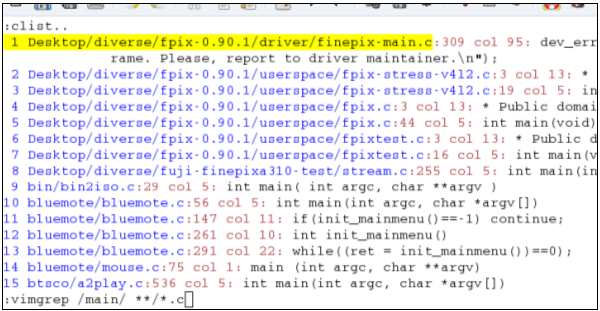
\includegraphics[scale=0.7]{./images/page66.png}
\end{center}
\marginpar{67}
\subsection{搜索帮助系统}
\label{subsec:search_the_help_system}

有时候需要从 Vim 中得到某些帮助信息, 此时用户可能并不确切地知道应该查找哪些信
息. 当然, 你可以在整个帮助系统中从头开始查找, 不过, Vim 的帮助系统包含众多的文
件, 以及数以千计的关键词.

为了解决这个问题, Vim 提供了一个专门的命令. 在前一节中, 我们用的是
\texttt{vimgrep}, 而对于 Vim 帮助系统, 则用的是下面这个命令:
\begin{vimcode}
:helpgrep pattern [@LANG]
\end{vimcode}
命令需要一个必填参数 --- 你所想要搜索的模式 --- 还有一个是可选参数, 用于限定语
言, 让我们来看一个例子. 比如说用户需要一些关于自动补全的帮助信息, 但是不知道
从哪里开始查找. 因为用户只了解英文, 所以你希望帮助信息也是英文的. 完成这个搜索
的命令是:
\begin{vimcode}
:helpgrep completion@en
\end{vimcode}
命令所执行的操作是在所有的英文 (\texttt{en}) 文档中搜索单词 \texttt{completion}.
搜索完成后, 光标会跳转到第一个匹配, 剩下的匹配结果则添加到 quickfix 列表, 以便
稍后检索.

\begin{warning}
    如果用户想使用 location 列表, 而不是 quickfix 列表, 就用 \texttt{:lhelpgrep}
    替换掉 \texttt{:helpgrep}.
\end{warning}

实际上, 命令 \texttt{helpgrep} 并没有遍历所有的文档, 而且使用了 tag list 来搜索
模式. tag list 并不会自动生成, 所以, 如果用户安装的插件带有自己的文档, 那就必须
使用下面的命令:
\begin{vimcode}
    :helptags /path/to/documentation
\end{vimcode}
把 \texttt{/path/to/documentation} 替换成新文档的安装位置, 但是为了能让 Vim 找
到文档, 新文档必须放在 Vim 选项 \texttt{runtimepath} 定义的几个目录的
\texttt{docs/} 子目录中 (参考 \texttt{:help 'runtimepath'}).
\marginpar{68}

\section{标记位置}
\label{sec:x_marks_the_spot}

有时, 当我们在编辑文件的某一行时, 需要跳到另一个地方查看一下. 之后, 我们可能很
难找到原来的那一行.

如果能在离开前作一下标记, 这样的话, 找到离开时的位置就方便多了.

为此, Vim 提供了一些工具用于完成这个功能. 这些工具可以分成两类:
\begin{itemize}
    \item 可见的标记
    \item 隐藏的标记
\end{itemize}

\subsection{可见的标记 --- 使用符号}
\label{subsec:visible_markers_using_signs}

在 Vim 中, 我们可以用一个可见的标记 --- 符号 --- 来标记一行. 一个符号指的是一
个标记, 它会显示在编辑器最靠左的列中.

\begin{warning}
    如果用户想改变显示符号的列的颜色, 可以使用下面这个命令:
    \begin{vimcode}
    :highlight SignColumn guibg=darkgrey
    \end{vimcode}
\end{warning}

根据所使用的 Vim 版本 (控制台或 GUI) 的不同, 符号或者是一些字符的组合 (比如
\texttt{>>}), 或者是一个图标. 为了使用符号, 需要作一些设置. 如果把设置信息写
在 \texttt{vimrc} 中, 就用不着每次都设置一遍.

第一件要做的事是定义你想用的符号. 定义符号的命令是:
\begin{vimcmdform}
\texttt{:sign define}\ \textit{name}\ \textit{arguments}
\end{vimcmdform}
\textit{arguments} 可以是下面几种之一:
\begin{itemize}
    \item \texttt{linehl}: 用于标记行的色彩组
    \item \texttt{text}: 该文本将作为符号, 显示在控制台 Vim 中 (比如
        \texttt{>>!!} 或 \texttt{++}). 每一个符号最多可以用两个字符.
    \item \texttt{texthl}: 用于标记符号文本的色彩组
    \item \texttt{icon}: 图标的完整路径, 该图标可用在 Gvim 的符号中. 图标应该
        足够小, 小到能够放到两个字符的空间中. 图标文件的格式可以是位图文件,
        不过最好是 \texttt{.xpm}.
\end{itemize}
\marginpar{69}
一个简单的例子是:
\begin{vimcode}
:sign define information text=!> linehl=Warning texthl=Error icon=/path/
to/information.xpm
\end{vimcode}
现在, 我们已经定义了一个符号, 并且把定义的命令添加到了 \texttt{vimrc} 中, 我们
已经准备好把该符号放到文件中的某个位置, 放置符号的命令是:
\begin{vimcode}
:exe ":sign place 123 line=" . line(.) ."name=information file=" .
expand("%:p") \end{vimcode}
用户可以把数字 \texttt{123} 替换成任意一个数字, 它将作为这个符号的 ID.

正如你所看到的那样, 放置符号的命令写起来有点麻烦, 但是我们可以把它映射到一
个键上.

命令的效果是把名字为 \texttt{information}, 且 ID 号为 \texttt{123} 的符号放置
到当前打开文件 (\verb'expand("%:p")') 的当前行 (\texttt{line(.)}). 映射的命令
是:
\begin{vimcode}
:map <F7> :exe ":sign place 123 line=" . line(".") ."name=infomation
file=" . expand("%:p")<CR>
\end{vimcode}
上面的命令把符号 \texttt{infomation} 映射到键 \key{F7}, 当你按下 \texttt{F7}
时, 符号就会被放置到当前行.
\begin{center}
    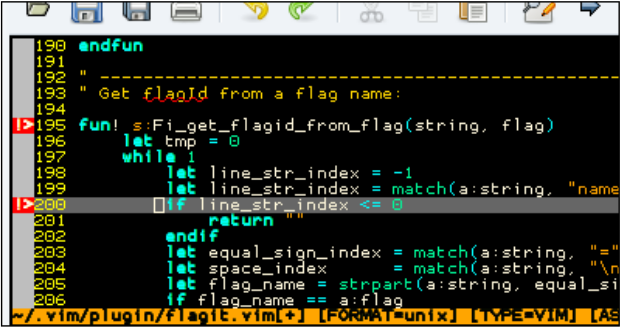
\includegraphics[scale=0.6]{./images/page69.png}
\end{center}
有时候, 我们想要移除符号, 用术语来讲, 叫作 ``unplace'' 一个符号:
\begin{vimcmdform}
\texttt{:sign unplace}\ \textit{ID}
\end{vimcmdform}
\marginpar{70}

命令中的 \textit{ID} 是放置符号时的 ID (在前面的例子中就是 \texttt{123}). 这个
命令会把所有的, 用该 ID 放置的符号移除. 用户可能只想把当前文件中的指定符号移
除, 这时候可以在命令的末尾加上另一个参数, 用来指定文件:
\begin{vimcmdform}
\texttt{:sign unplace}\ \textit{ID}\ \texttt{file=}\textit{name}
\end{vimcmdform}
或者用下面这个命令从当前缓冲区中移除符号:
\begin{vimcmdform}
\texttt{:sign unplace}\ \textit{ID}\ \texttt{buffer=}\textit{bufferno}
\end{vimcmdform}
命令中的 \textit{bufferno} 是当前缓冲区的编号 (可以通过命令 \texttt{:buffers}
查看).

如果只想移除当前行的符号, 用:
\begin{vimcode}
:sign unplace
\end{vimcode}
为了和放置符号的按键映射相对应, 我们可以把它映射到 \key{Ctrl+F7} 上:
\begin{vimcode}
:map <C-F7> :sign unplace<CR>
\end{vimcode}

\begin{warning}
    如果你在同一个文件中, 用同一个 ID 添加了多个符号, 那么上面的命令只会移除
    文件内最靠前的符号, 而非当前行的符号.
\end{warning}

既然本章讨论的是导航, 那么我们也要介绍一下如何跳转到一个符号. 这种跳转在 Vim 中
称为 符号跳转 (sign-jumping), 所使用的命令是:
\begin{vimcmdform}
\texttt{:sign jump}\ \textit{ID}\ \texttt{file=}\textit{file}
\end{vimcmdform}
命令中的 \textit{ID} 是你想要跳转到的符号 ID, \textit{file} 指定在哪个文件中
搜索该符号. 除了 \texttt{file=}\textit{file}, 还可以用 \texttt{buffer=}%
\textit{bufferno}.

同样, 如果在同一个文件/缓冲区内用同一个 ID 添加了多个符号, 那么命令只能跳转到
该 ID 在文件内的第一个符号.

\begin{warning}
    Paul Rouget 开发了一个 Vim 脚本, 通过它我们可以非常方便地使用符号. 脚本的
    下载地址是 \url{http://www.vim.org/scripts/script.php?script_id=1580}.
\end{warning}
\marginpar{71}

\subsection{隐藏的标记}
\label{subsec:hidden_markers_using_marks}

为了给当前行作标记, 我们可以使用标记 (mark). 它的使用方法非常简单, 总的来说,
它由两个在普通模式下使用的命令组成, 一个用于设置标记, 另一个用于跳转到标记.
除非打开标记列表, 否则用户无法判断某一行是否含有标记.

我们首先来看一下如何标记当前行. 为了标记当前行, 我们只需要在普通模式下按下
\texttt{m}, 后面再紧跟着某个字符, 这个字符可以是 \texttt{0}-\texttt{9},
\texttt{a}-\texttt{z},或 \texttt{A}-\texttt{Z} 中的一个. 例如, 如果用户执行
了 \texttt{ma}, 那就是说用名字为 \texttt{a} 的标记来标记当前行. 然后, 如果用户
想要跳转到标记 \texttt{a} 所在的行, 只需要按下 \texttt{'a} (单引号 + 标记名),
光标就会马上跳转到该行的开始 (如果该行是缩进过的, 那就跳转到该行的第一个非空白字
符).

有时候, 光是跳转到一行的开始可能还不够, 如果能直接跳转到添加标记时光标所在的具
体位置可能会更好一点. 为了达到这个目的, 需要把跳转命令中的单引号改成反单引号
(\texttt{`}), 于是, 跳转到标记 \texttt{a} 的命令就变成了 \texttt{`a}.

不同的标记名含有不同的意义, 它们的使用范围如下所示:
\begin{center}
    \begin{tabular}{lp{40em}}
    \hline
    标记        & 用法 \\
    \hline
    \texttt{0}-\texttt{9} & 这个标记集来源于文件 \texttt{.viminfo}, 通常保留
    给 Vim 内部使用 (比如, 标记 \texttt{0} 表示文件最后一次退出时, 光标所在的
    位置. 然而, 用户可以利用这些标记来实现 ``打开最近使用过的文件''. \\
    \texttt{a}-\texttt{z} & 这些标记只在当前文件内有效, 当文件关闭时删除这些
    标记. 如果用户此时是在当前文件的缓冲区内, 那么只能通过这些小写字母标记在
    文件内跳转. \\
    \texttt{A}-\texttt{Z} & 这些标记可以跨越文件使用. 即使没有打开目的标记所在
    的文件, 也可以直接跳转到标记所在的位置. 如果 \texttt{.viminfo} 文件是可用
    的, 那么这些标记就会被保存下来, 直到下一次对文件进行编辑. \\
    \hline
\end{tabular}
\end{center}

用户可以通过下面这个命令来获取完整的, 正在使用的标记列表:
\begin{vimcode}
:marks
\end{vimcode}
命令显示了每个标记所在的文件与行号. 为了删除一个或多个标记, 执行:
\begin{vimcmdform}
\texttt{:delmarks}\ \textit{markid markid...markid}
\end{vimcmdform}
具体的使用例子有:
\begin{vimcode}
:delmarks a b c
:delmarks a-c
:delmarks a f-i 1-4
\end{vimcode}
\marginpar{72}
如果用户想要删除当前缓冲区内的所有标记, 执行:
\begin{vimcode}
:delmarks!
\end{vimcode}

当使用 Vim 时, 它会自动设置其他类型的标记. 其他类型的标记包括但不限于: 最后
一次退出插入模式时光标所在的位置; 可视模式下被选中的文本的开始与结束; 最后一
次被修改的地方.

关于如何使用标记, 以及其他类型标记的更多信息, 参考 \texttt{:help mark-motions}.

\section{小结}
\label{sec:better_navigation_summary}

在这一章, 我们介绍了在文件与缓冲区内快速导航的方法.

首先, 我们介绍了如何根据文件的上下文结构, 在文件内部快速导航. 除此之外, 还讨论了
如何在冗长并且折叠过的行中移动光标.

然后, 我们介绍了如何在 Vim 的帮助系统中导航, 还学习到了如何通过简单的按键绑定,
使得导航更加直观, 便于记忆.

既然我们已经知道了如何在文件内导航, 还要知道如何在多个文件与多个缓冲区之间导航.
再接下来的小节我们学习了如何快速地在缓冲区之间导航, 以及如何通过两次击键, 来
打开被另一个文件所引用的文件.

导航的方式有许多种, 再接下来的小节我们学习到利用搜索, 不仅可以在打开的文件内
导航, 甚至包括磁盘上的文件. 我们还学习了如何在 Vim 的帮助系统搜索某个主题的相
关帮助信息.

最后, 我们学习了如何通过符号与标记在文件间跳转, 以及当我们使用 Vim 时, 它会如何
自动地帮助我们添加标记.

我们已经学习到了如何在 Vim 中迅速地导航, 可以继续阅读下一章节. 在下一章里, 我
们会用到更多的 Vim 内置功能 来提高工作效率.
